\documentclass[UTF8,12pt,a4paper]{ctexart}
\usepackage{amsmath,amssymb,bm}
\usepackage{booktabs}
\usepackage{graphicx}
\usepackage{geometry}
\usepackage{float}
\usepackage{hyperref}
\usepackage{xcolor}
\geometry{left=2.3cm,right=2.3cm,top=2.5cm,bottom=2.5cm}
\hypersetup{colorlinks=true,linkcolor=blue!45!black,urlcolor=blue!55!black}
\setlength{\parindent}{2em}
\setlength{\parskip}{0.25em}
\graphicspath{{./}}

\title{\textbf{七杆闭链机构中 1--3--5--7 平面四杆模式\\显式解与傅里叶拟合报告}}
\author{}
\date{\today}

\begin{document}
\maketitle
\tableofcontents
\newpage

\begin{abstract}
本文针对一类七转动关节闭链机构，研究关节3、5、7锁定在初始角度、关节2、4、6、1保持轴线平行时形成的平面四杆运动模式。计算严格沿用原程序中的改进DH变换，并以零关节变量构型为初始闭环姿态。通过提取四根活动轴的轴心，空间闭环被约化为平面四杆的两圆交点问题，由此获得关节4、6、1关于输入角$q_2$的几何显式解。该解在$q_2\in[0,2\pi]$的721个采样点上全部可达，代回完整七杆DH闭环后的最大位置误差为$5.930\times10^{-15}$，最大姿态误差为$5.376\times10^{-16}\,\mathrm{rad}$。进一步采用含线性斜率项的五阶傅里叶级数拟合显式解。三个活动从动关节的最大角误差不超过$0.1061^\circ$，说明该模型可作为高精度工程近似，但并非与显式解数学等价。
\end{abstract}

\section{问题定义}

七杆机构的DH参数按
\[
[\alpha_{r-1},a_{r-1},d_r,\theta_{r,\mathrm{offset}}]
\]
排列。这里只改变关节名称，后续变换矩阵中的$r=1,\ldots,7$仍表示闭环连乘的链位置；链位置对应的新关节编号依次为$2,3,4,5,6,7,1$，如表\ref{tab:dh}所示。

\begin{table}[H]
\centering
\caption{七杆机构的改进DH参数}
\label{tab:dh}
\begin{tabular}{ccccc}
\toprule
新关节编号 & $\alpha$ & $a$ & $d$ & $\theta_{\mathrm{offset}}$\\
\midrule
2 & $0$ & $l$ & $0$ & $0$\\
3 & $\pi/2$ & $2l$ & $2.5l$ & $0$\\
4 & $\pi/2$ & $0$ & $0$ & $\pi$\\
5 & $\pi/2$ & $2.5l$ & $0$ & $0$\\
6 & $\pi/2$ & $2.5l$ & $0$ & $0$\\
7 & $\pi/2$ & $0$ & $2.5l$ & $\pi$\\
1 & $\pi/2$ & $2l$ & $0$ & $0$\\
\bottomrule
\end{tabular}
\end{table}

实际DH转角为
\[
\theta_r=q_{\nu(r)}+\theta_{r,\mathrm{offset}},\qquad \nu(r)=(2,3,4,5,6,7,1)_r.
\]
初始关节变量为
\[
\bm q_0=[0,0,0,0,0,0,0]^{\mathsf T}.
\]
因此，第4、7关节的初始实际DH转角仍包含参数表中的$\pi$偏置。平面模式的一般锁定条件为
\[
q_3=q_{3,0},\qquad q_5=q_{5,0},\qquad q_7=q_{7,0},
\]
本算例恰有$q_{3,0}=q_{5,0}=q_{7,0}=0$。

\section{改进DH闭环}

单节变换矩阵为
\[
{}^{r-1}T_r=
\begin{bmatrix}
\cos\theta_r&-\sin\theta_r&0&a_{r-1}\\
\sin\theta_r\cos\alpha_{r-1}&\cos\theta_r\cos\alpha_{r-1}&-\sin\alpha_{r-1}&-d_r\sin\alpha_{r-1}\\
\sin\theta_r\sin\alpha_{r-1}&\cos\theta_r\sin\alpha_{r-1}&\cos\alpha_{r-1}&d_r\cos\alpha_{r-1}\\
0&0&0&1
\end{bmatrix}.
\]
完整闭环条件为
\[
T_{\mathrm{end}}(\bm q)=\prod_{r=1}^{7}{}^{r-1}T_r=I_4.
\]
初始构型满足
\[
\|T_{\mathrm{end}}(\bm q_0)-I_4\|_F=9.87\times10^{-16},
\]
因此可作为解析运动的出发位置。

\section{平面四杆约化}

按照改进DH变换的实际转轴位置计算关节轴心，关节2、4、6、1在初始公共平面内的坐标为
\[
P_2=(1,0),\quad P_4=(3,-2.5),\quad
P_6=(-2,-2.5),\quad P_1=(0,0).
\]
对应四杆长度为
\[
L_{24}=L_{61}=\frac{\sqrt{41}}{2}l,\qquad
L_{46}=5l,\qquad L_{12}=l.
\]
以关节2轴线方向为公共平面法向，四根活动轴的方向符号为
\[
[\sigma_2,\sigma_4,\sigma_6,\sigma_1]=[1,-1,1,1].
\]

\section{轴心位置的显式解}

令$\Delta q_2=q_2-q_{2,0}$。关节4的轴心位置为
\[
P_4(q_2)=P_2+R(\sigma_2\Delta q_2)(P_{4,0}-P_2),
\]
其中
\[
R(\psi)=
\begin{bmatrix}
\cos\psi&-\sin\psi\\
\sin\psi&\cos\psi
\end{bmatrix}.
\]
关节6轴心满足
\[
\|P_6-P_4\|=L_{46},\qquad \|P_6-P_1\|=L_{61}.
\]
定义
\[
D=\|P_1-P_4\|,\qquad
\bm e=\frac{P_1-P_4}{D},\qquad
\bm e_\perp=(-e_y,e_x),
\]
则两圆交点显式写为
\[
P_6=P_4+x\bm e+s\,h\bm e_\perp,
\]
其中
\[
x=\frac{L_{46}^{2}-L_{61}^{2}+D^{2}}{2D},
\qquad
h=\sqrt{L_{46}^{2}-x^{2}},
\qquad s\in\{-1,+1\}.
\]
$s$对应两条装配支路。通过初始点$P_{6,0}$选择本算例的$s=+1$。当$h^2<0$时输入角不可达；本算例整周无不可达点。

\section{DH关节角显式回映射}

定义三根活动杆的绝对方向
\[
\phi_{24}=\operatorname{atan2}(P_{4y}-P_{2y},P_{4x}-P_{2x}),
\]
\[
\phi_{46}=\operatorname{atan2}(P_{6y}-P_{4y},P_{6x}-P_{4x}),
\]
\[
\phi_{61}=\operatorname{atan2}(P_{1y}-P_{6y},P_{1x}-P_{6x}).
\]
记$\Delta\phi_{jk}=\phi_{jk}-\phi_{jk,0}$，并沿运动序列连续展开角度，则
\[
\Delta q_4=\frac{\Delta\phi_{46}-\sigma_2\Delta q_2}{\sigma_4},
\]
\[
\Delta q_6=\frac{\Delta\phi_{61}-\sigma_2\Delta q_2-\sigma_4\Delta q_4}{\sigma_6},
\]
\[
\Delta q_1=-\frac{\sigma_2\Delta q_2+\sigma_4\Delta q_4+\sigma_6\Delta q_6}{\sigma_1}.
\]
代入本算例的轴方向符号，得到
\[
q_4(q_2)=\Delta q_2-\Delta\phi_{46},
\]
\[
q_6(q_2)=\Delta\phi_{61}-\Delta q_2+q_4,
\]
\[
q_1(q_2)=-\Delta q_2+q_4-q_6.
\]
由于$\phi_{46}$与$\phi_{61}$中的$P_6$已由两圆交点公式显式给出，上述关系构成关于$q_2$的闭式几何表达，而不是数值优化或曲线拟合结果。

\section{数值结果与完整闭环验证}

在$q_2\in[0,2\pi]$上均匀选取721个采样点，所有输入角均存在当前装配支路的实数解。代表位置列于表\ref{tab:result}。

\begin{table}[H]
\centering
\caption{代表输入位置的DH关节角}
\label{tab:result}
\begin{tabular}{rrrr}
\toprule
$q_2$ & $q_4$ & $q_6$ & $q_1$\\
\midrule
$0^\circ$   & $0.000^\circ$ & $0.000^\circ$ & $0.000^\circ$\\
$45^\circ$  & $10.289^\circ$ & $5.234^\circ$ & $-39.945^\circ$\\
$90^\circ$  & $20.521^\circ$ & $2.257^\circ$ & $-71.736^\circ$\\
$135^\circ$ & $28.609^\circ$ & $-8.021^\circ$ & $-98.369^\circ$\\
$180^\circ$ & $32.990^\circ$ & $-22.335^\circ$ & $-124.675^\circ$\\
$225^\circ$ & $26.868^\circ$ & $-32.856^\circ$ & $-165.276^\circ$\\
$270^\circ$ & $4.010^\circ$ & $-26.272^\circ$ & $-239.717^\circ$\\
$315^\circ$ & $-5.318^\circ$ & $-11.849^\circ$ & $-308.469^\circ$\\
$360^\circ$ & $0.000^\circ$ & $0.000^\circ$ & $-360.000^\circ$\\
\bottomrule
\end{tabular}
\end{table}

\begin{figure}[H]
\centering
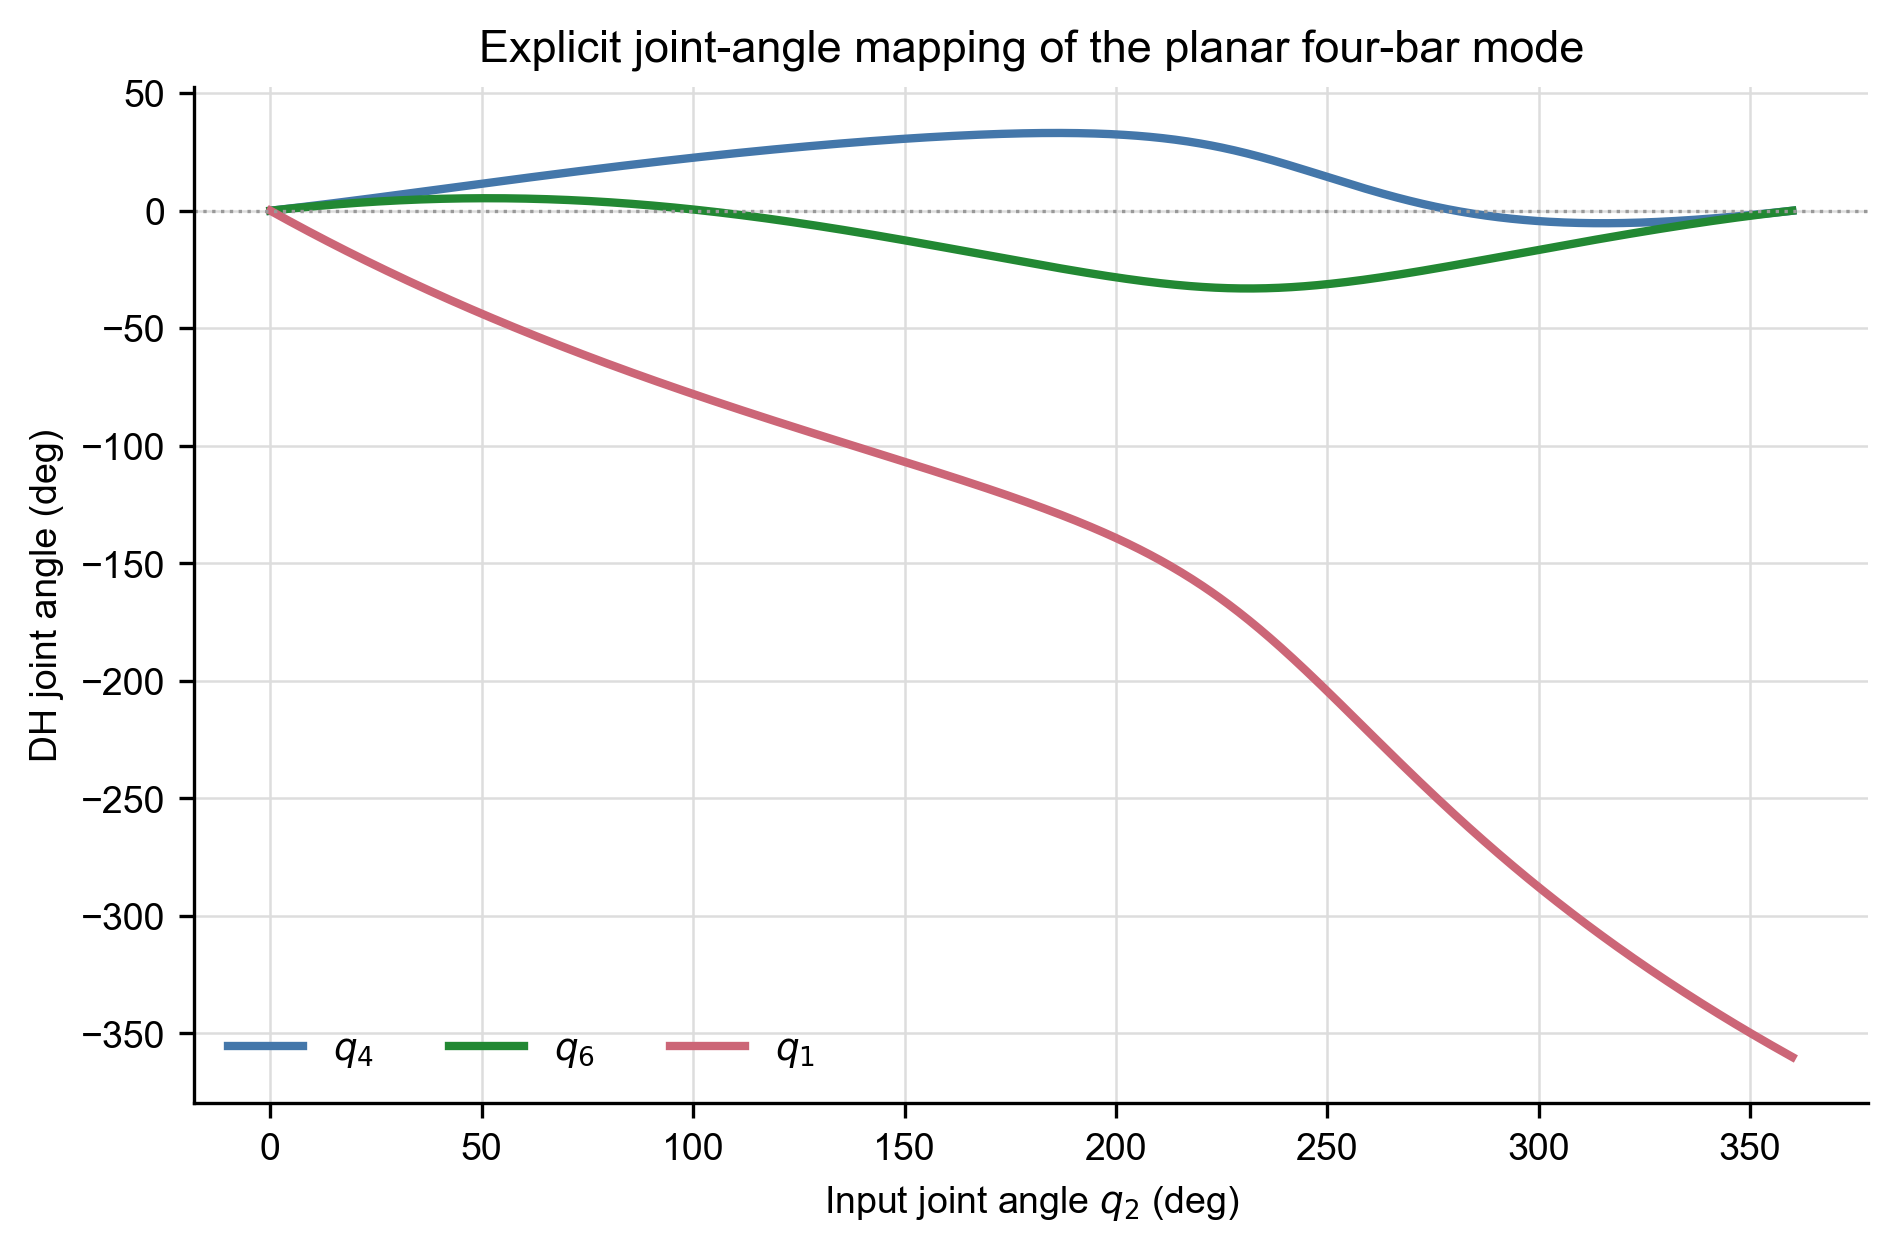
\includegraphics[width=0.92\textwidth]{explicit_solution/joint_angle_mapping.png}
\caption{平面四杆运动模式下的关节角显式解。}
\end{figure}

将每组显式解代回完整七杆DH矩阵，得到
\[
\max e_p=5.930\times10^{-15},\qquad
\max e_R=5.376\times10^{-16}\ \mathrm{rad}.
\]
误差处于双精度浮点舍入量级。

\begin{figure}[H]
\centering
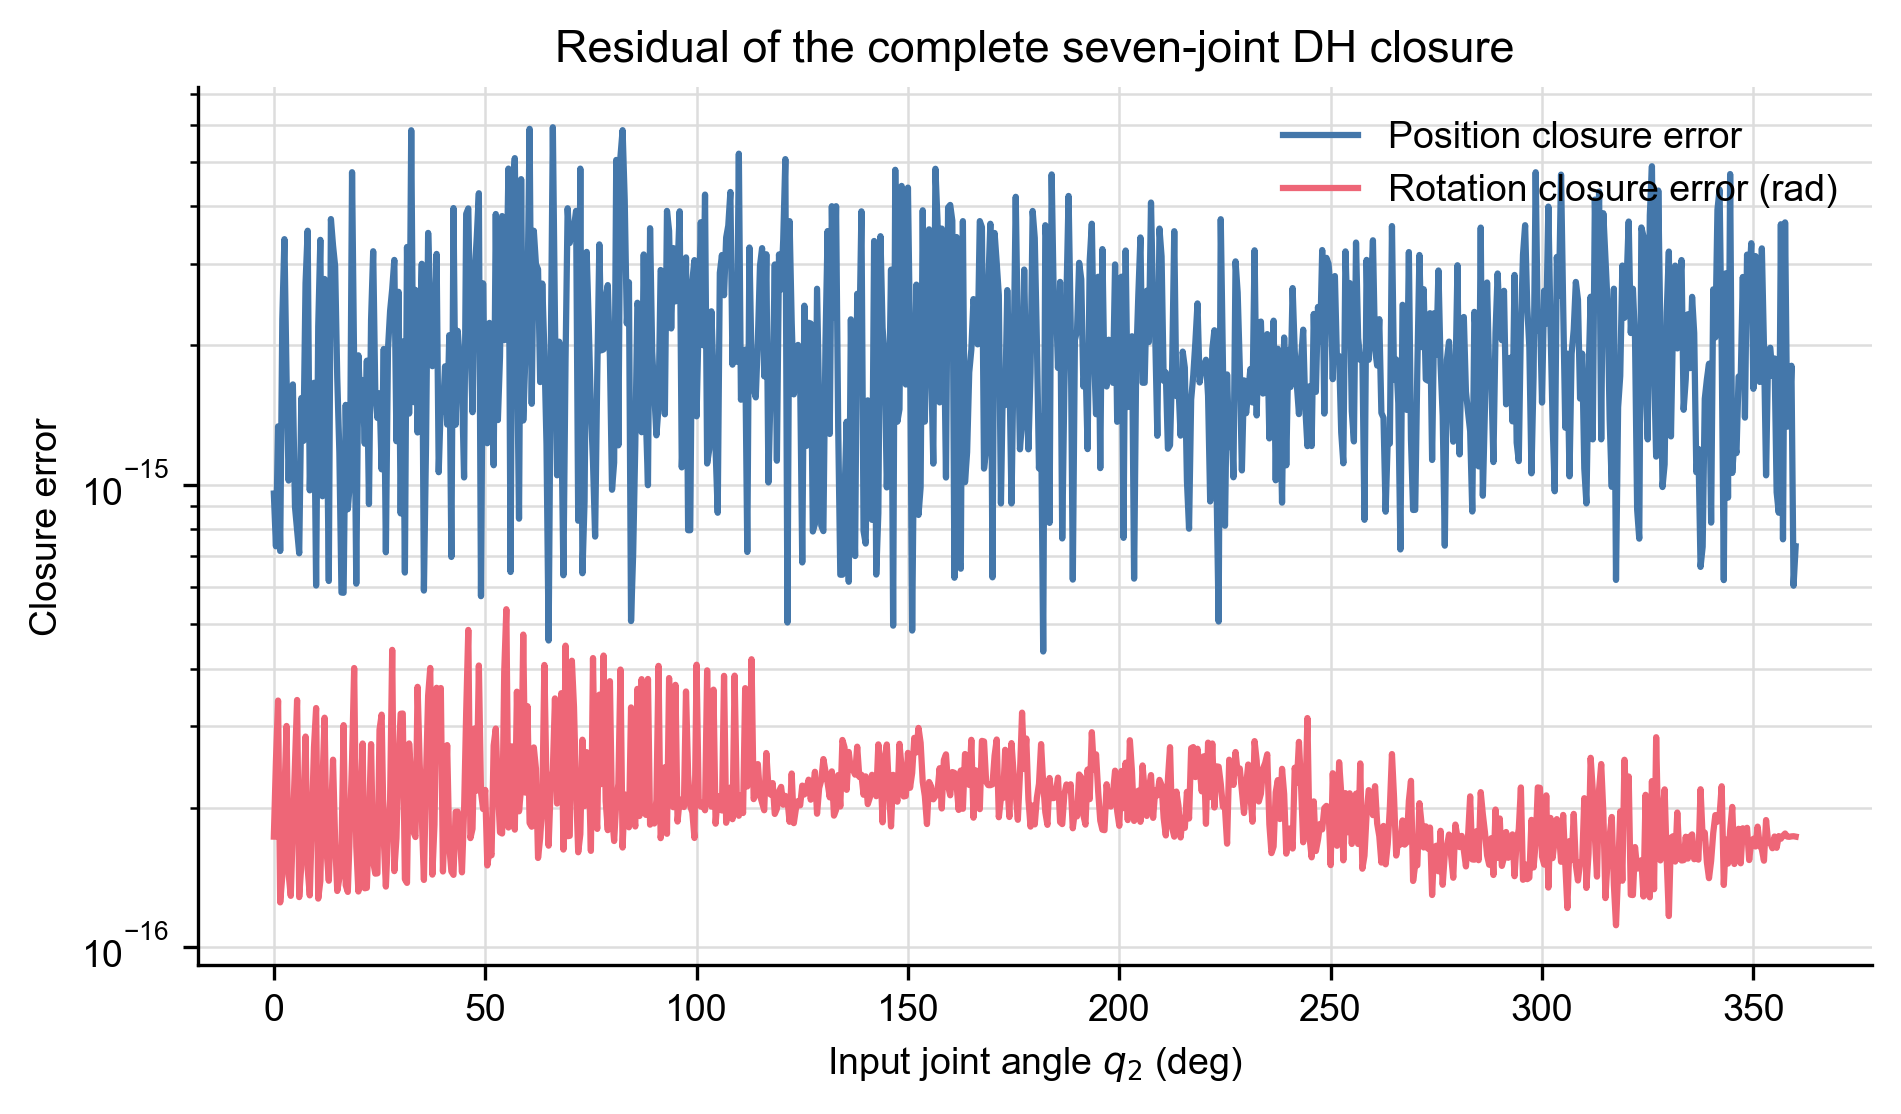
\includegraphics[width=0.88\textwidth]{explicit_solution/closure_error.png}
\caption{显式解代回完整七杆DH方程后的闭环误差。}
\end{figure}

\begin{figure}[H]
\centering
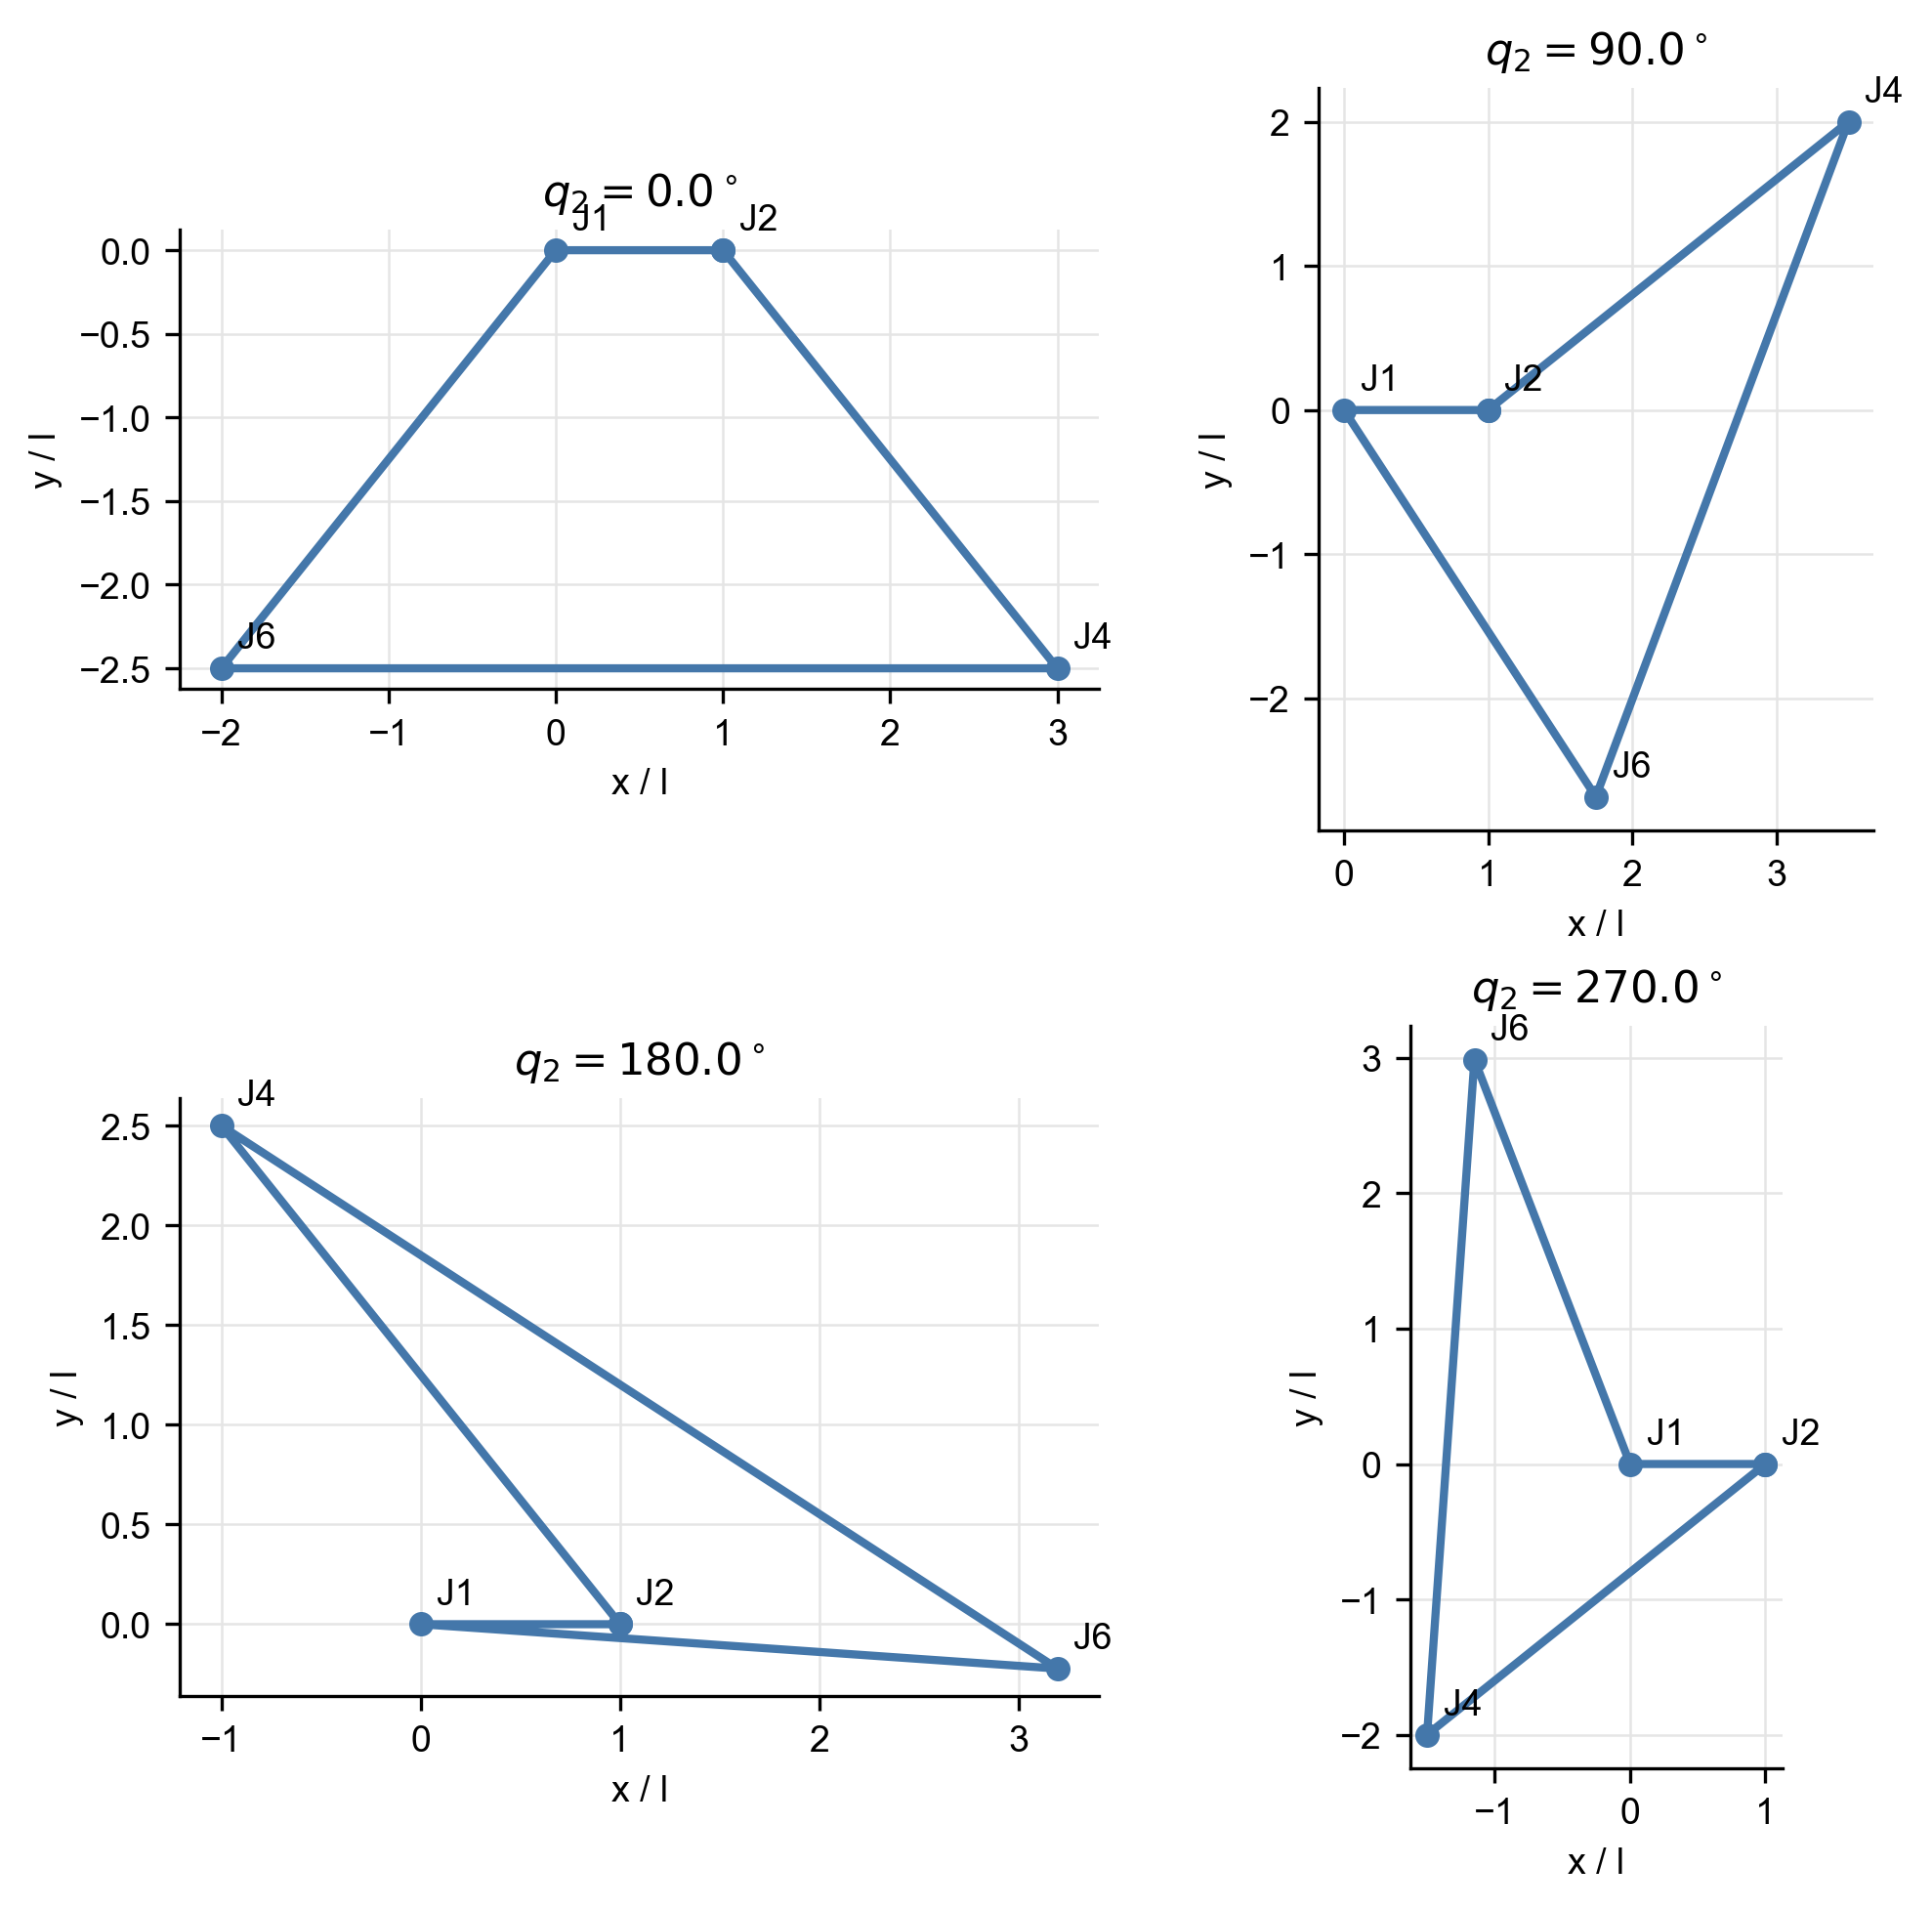
\includegraphics[width=0.82\textwidth]{explicit_solution/fourbar_configurations.png}
\caption{四个典型输入角下的平面四杆构型。}
\end{figure}

\section{带斜率五阶傅里叶拟合}

由于$q_1$在输入转动一周后累计变化约$-2\pi$，采用含线性斜率项的广义五阶傅里叶模型
\[
\widehat q_i(x)=c_{0,i}+c_{1,i}x+
\sum_{k=1}^{5}\left[a_{k,i}\cos(kx)+b_{k,i}\sin(kx)\right],
\qquad x=q_2.
\]
主要拟合系数列于表\ref{tab:coef}，完整系数见结果目录中的CSV文件。

\begin{table}[H]
\centering
\caption{带斜率五阶傅里叶模型的部分系数（rad）}
\label{tab:coef}
\resizebox{\textwidth}{!}{
\begin{tabular}{rrrrrrr}
\toprule
关节 & $c_0$ & $c_1$ & $a_1$ & $b_1$ & $a_2$ & $b_2$\\
\midrule
$q_4$ & 0.256376 & 0.000288 & -0.299473 & 0.126236 & 0.036554 & 0.060048\\
$q_6$ & -0.204336 & -0.000115 & 0.203030 & 0.253558 & 0.007546 & -0.033653\\
$q_1$ & 0.460713 & -0.999597 & -0.502502 & -0.127322 & 0.029009 & 0.093701\\
\bottomrule
\end{tabular}}
\end{table}

\begin{table}[H]
\centering
\caption{五阶傅里叶模型相对显式解的角度误差}
\begin{tabular}{rrrr}
\toprule
关节 & RMSE & 最大绝对误差 & $R^2$\\
\midrule
$q_4$ & $0.03453^\circ$ & $0.07361^\circ$ & 0.999993447\\
$q_6$ & $0.01519^\circ$ & $0.03274^\circ$ & 0.999998684\\
$q_1$ & $0.04954^\circ$ & $0.10609^\circ$ & 0.999999771\\
\bottomrule
\end{tabular}
\end{table}

\begin{figure}[H]
\centering
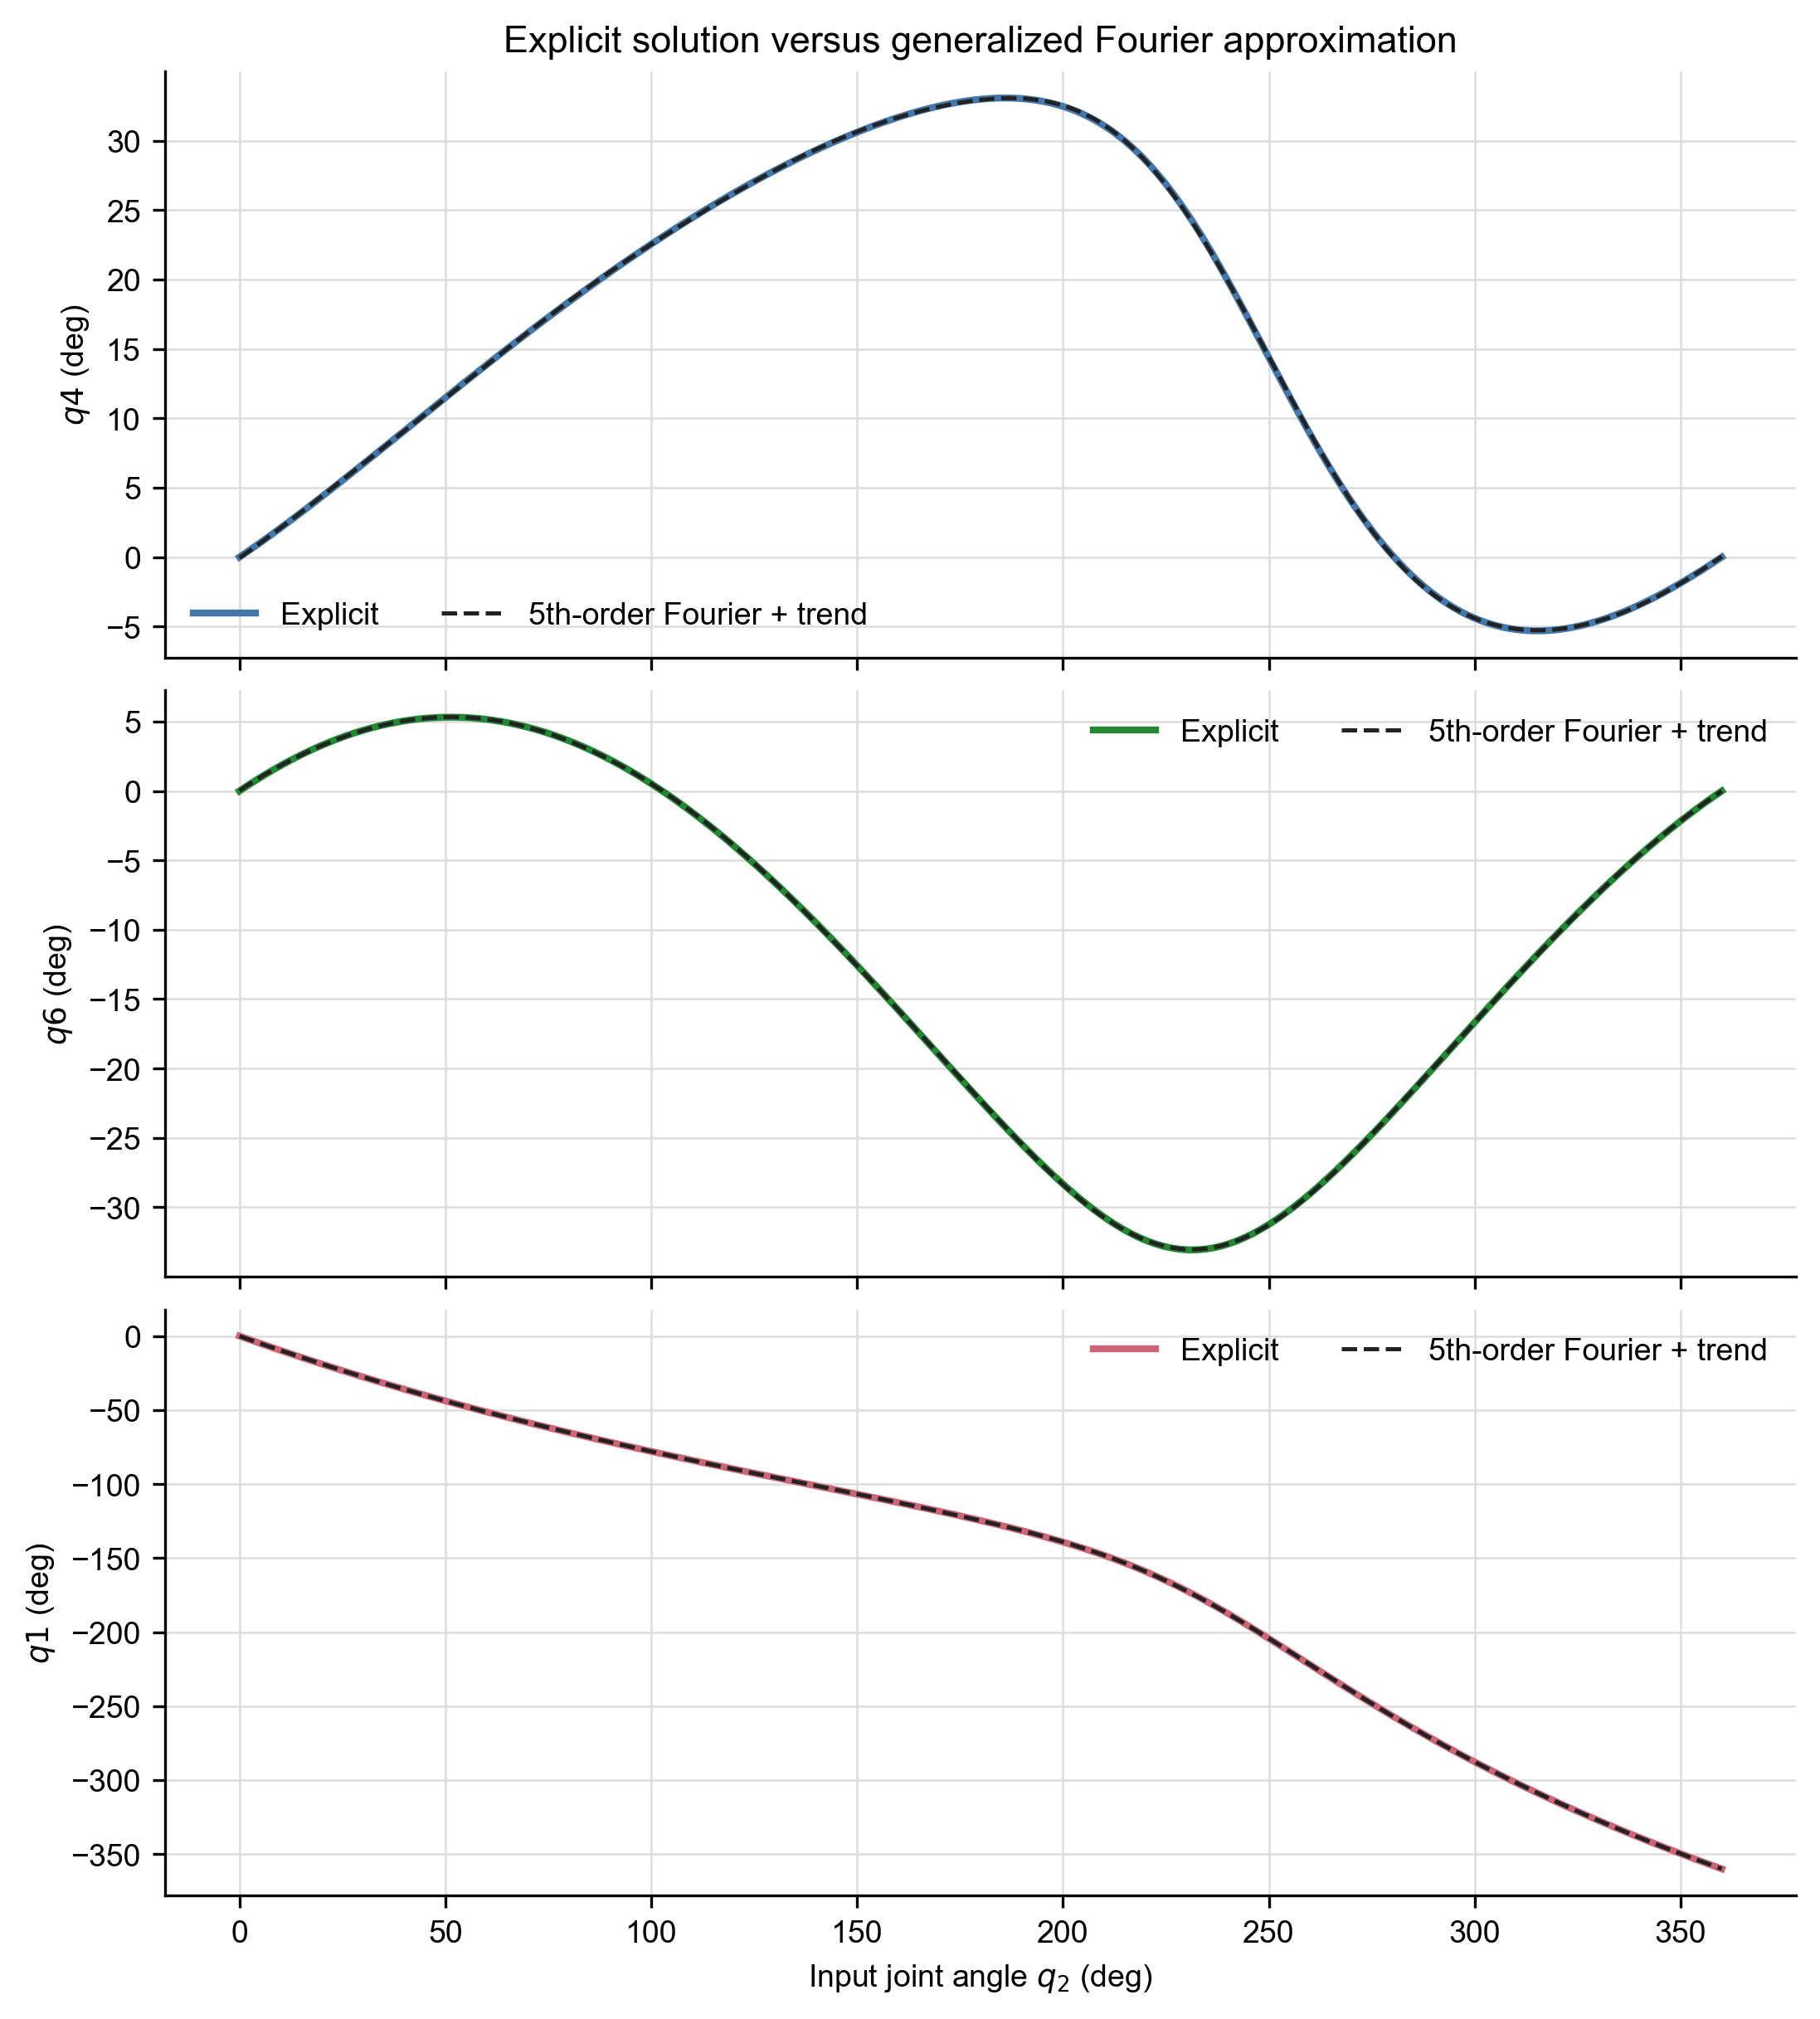
\includegraphics[width=0.92\textwidth]{fourier_comparison/explicit_vs_fourier.png}
\caption{几何显式解与带斜率五阶傅里叶模型的对比。}
\end{figure}

\begin{figure}[H]
\centering
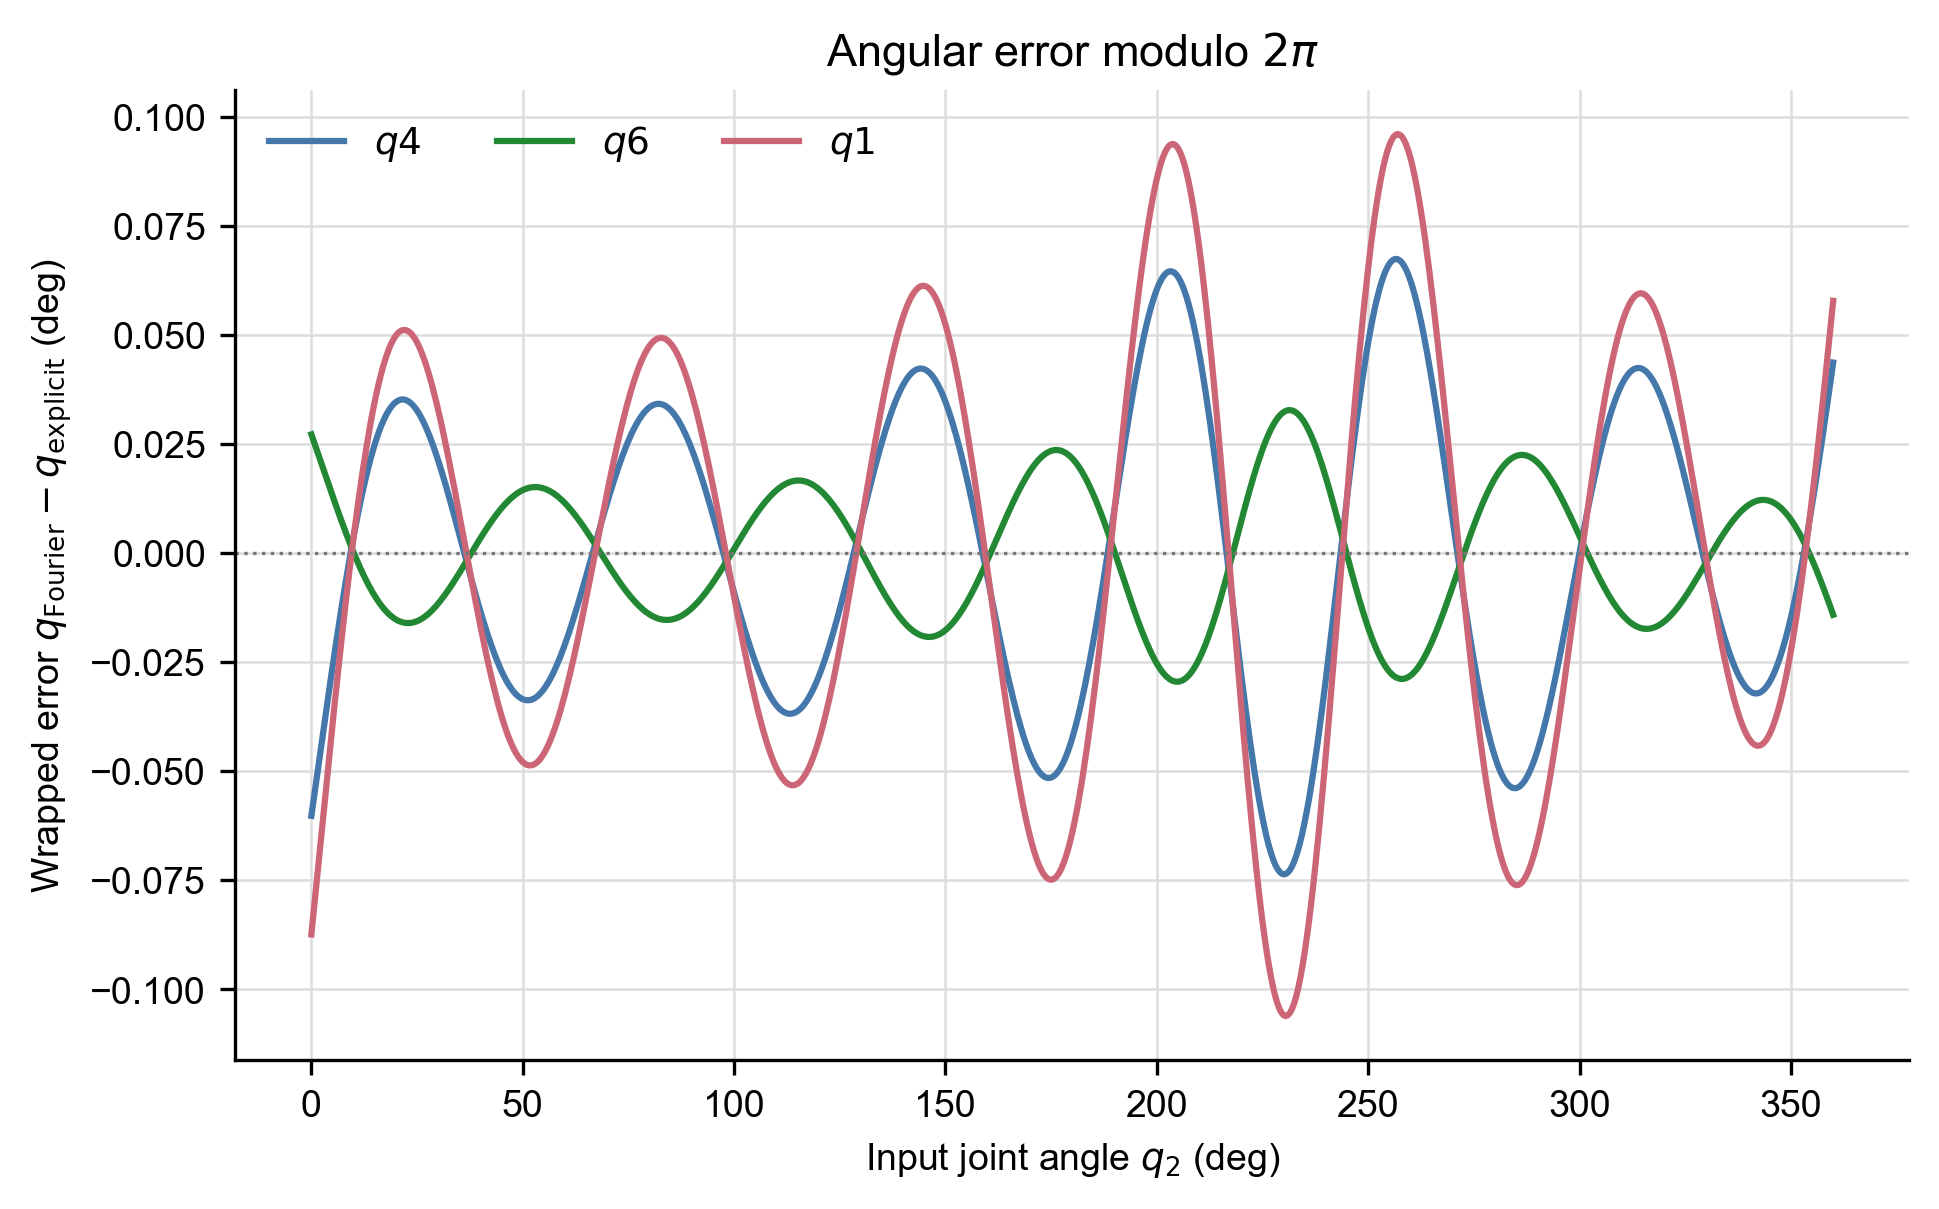
\includegraphics[width=0.90\textwidth]{fourier_comparison/fourier_error.png}
\caption{傅里叶拟合相对显式解的模$2\pi$角度误差。}
\end{figure}

将傅里叶拟合角代回完整七杆DH方程，最大位置闭环误差为
\[
4.4047\times10^{-3}l,
\]
最大姿态闭环误差为
\[
5.2619\times10^{-15}\ \mathrm{rad}.
\]
姿态误差仍接近零，是因为四个活动关节角之间的总转角关系被线性基函数保持；位置误差不为零，说明有限阶傅里叶模型没有严格满足两圆位置闭环。

\section{结论与使用边界}

\begin{enumerate}
\item 锁定关节3、5、7后，关节2、4、6、1的运动可由平面四杆两圆交点显式求解。
\item 得到的关节角不是平面杆件绝对角，而是经过轴方向符号换算后的原七杆DH变量。
\item 显式解代回完整七杆DH方程后的误差处于$10^{-15}$量级，可作为严格运动学解使用。
\item 带斜率五阶傅里叶级数与显式解在图像上高度重合，最大角误差约$0.1061^\circ$，可用于快速估计、控制器近似或曲线表达。
\item 傅里叶式并非与显式解完全相同。涉及精确闭环、奇异性分析或高精度轨迹生成时，应采用几何显式解。
\end{enumerate}

\section{结果文件}

\begin{itemize}
\item 显式解逐点数据：\texttt{explicit\_solution/joint\_angles.csv}
\item 显式解矢量图：\texttt{joint\_angle\_mapping.pdf}和\texttt{.svg}
\item 傅里叶逐点对比：\texttt{fourier\_comparison/explicit\_vs\_fourier.csv}
\item 傅里叶完整系数：\texttt{fourier\_comparison/fourier\_coefficients.csv}
\item 傅里叶误差指标：\texttt{fourier\_comparison/fourier\_error\_metrics.csv}
\item 程序目录：\texttt{E:/hub/planar\_fourbar\_dh}
\end{itemize}

\end{document}
